\section{TEXT Add Text Label to Plot}

\subsection{Usage}

Adds a text label to the currently active plot.  The general
syntax for it is use is either
\begin{verbatim}
   text(x,y,'label')
\end{verbatim}
where \verb|x| and \verb|y| are both vectors of the same length, in which
case the text \verb|'label'| is added to the current plot at each of the
coordinates \verb|x(i),y(i)| (using the current axis to map these to screen
coordinates).  The second form supplies a cell-array of strings
as the second argument, and allows you to place many labels simultaneously
\begin{verbatim}
   text(x,y,{'label1','label2',....})
\end{verbatim}
where the number of elements in the cell array must match the size of
vectors \verb|x| and \verb|y|.  You can also specify properties for the labels
via
\begin{verbatim}
   handles = text(x,y,{labels},properties...)
\end{verbatim}
\subsection{Example}

Here is an example of a few labels being added to a random plot:
\begin{verbatim}
--> plot(rand(1,4))
--> text([2,3],[0.5,0.5],{'hello','there'})
\end{verbatim}


\centerline{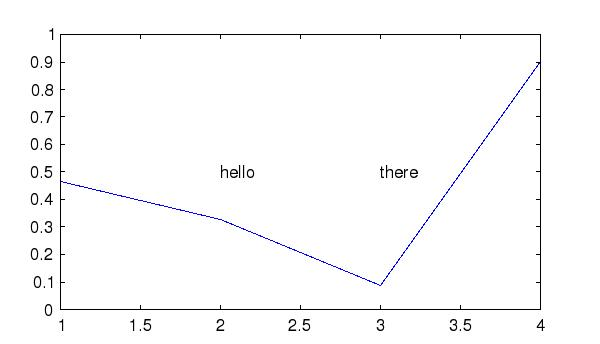
\includegraphics[width=8cm]{text1}}

Here is the same example, but with larger labels:
\begin{verbatim}
--> plot(rand(1,4))
--> text([2,3],[0.5,0.5],{'hello','there'},'fontsize',20)
\end{verbatim}


\centerline{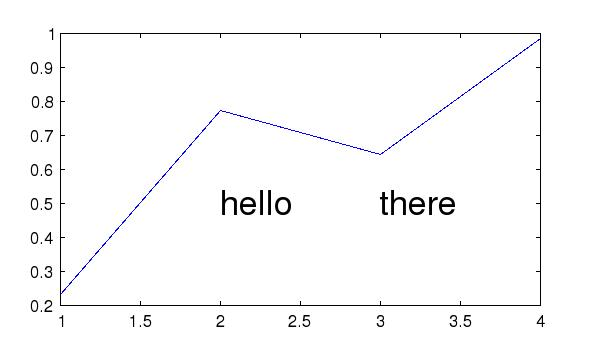
\includegraphics[width=8cm]{text2}}

